% Settings for the default beamer theme
\documentclass[english, aspectratio=169]{beamer}
\usepackage[T1]{fontenc}
\usepackage[utf8]{inputenc}
\usepackage{tabularx}
\usepackage{babel}
\usepackage[ruled,vlined]{algorithm2e}
\SetAlgorithmName{Algoritmus}{algoritmus}{List of Algorithms}
\setcounter{secnumdepth}{3}
\setcounter{tocdepth}{3}

\makeatletter

\newcommand\makebeamertitle{\frame{\maketitle}}

% (ERT) argument for the TOC
\AtBeginDocument{%
  \let\origtableofcontents=\tableofcontents
  \def\tableofcontents{\@ifnextchar[{\origtableofcontents}{\gobbletableofcontents}}
  \def\gobbletableofcontents#1{\origtableofcontents}
}

% Theme settings
\usetheme{Frankfurt}
\usecolortheme{default}
\usefonttheme[onlymath]{serif}

% Template settings
\setbeamertemplate{navigation symbols}{}
\setbeamertemplate{blocks}[rounded][shadow=false]
\setbeamertemplate{title page}[default][colsep=-4bp, rounded=true, shadow=false]
\makeatother

% Define a custom darker red color
\definecolor{DarkerRed}{RGB}{139,0,0} % Adjust the RGB values as needed

% Use the newly defined color in Beamer theme elements
\setbeamercolor{structure}{fg=DarkerRed} % Changes basic structural elements to Darker Red
\setbeamercolor{title in head/foot}{bg=DarkerRed} % Changes the title in header/footer to Darker Red


\begin{document}

% Title page
\section{Bevezetés}
\title[]{Üzleti Elemzések Módszertana}
\subtitle{4. Gyakorlat: Döntési fák}
\author[Kuknyó Dániel]{Kuknyó Dániel\\Budapesti Gazdasági Egyetem}
\date{2023/24\\2.félév}
\makebeamertitle

% Table of contents slide
\begin{frame}
\tableofcontents{}
\end{frame}

% Table of contents of the current section
\begin{frame}
\tableofcontents[currentsection]
\end{frame}

\begin{frame}{Döntési fák a gépi tanulásban}
\begin{columns}
\begin{column}{.5\textwidth}
A döntési fák olyanok, mint a svájci bicska: nagyon sok mindenre jó, de szinte semmire sem a legalkalmasabb.\par\medskip
A döntési fák kifejezetten hasznosak gyors taníthatóságuk, jól értelmezhetőségük és pontosságuk miatt.
\end{column}
\begin{column}{.5\textwidth}
\begin{center}

\includegraphics[width=5cm, height=7cm, keepaspectratio]{images/decision_trees_1.png}
\end{center}
\end{column}
\end{columns}
\end{frame}

\begin{frame}{Döntési fák alapjai}
\begin{columns}
\begin{column}{.5\textwidth}
A döntési fák képesek mind regressziós és osztályozási problémákat is végrehajtani. Könnyen illeszthetők komplex adathalmazokra.\par\medskip
Az algoritmus alapja, hogy \textbf{mintaegyedeket osztályoz változóikban felvett értékeik alapján}. 
\end{column}
\begin{column}{.5\textwidth}
\begin{center}

\includegraphics[width=7cm, height=7cm, keepaspectratio]{graphs/decision_trees_1.png}
\end{center}
\end{column}
\end{columns}
\end{frame}

\begin{frame}{Egy kezdeti döntési fa}
\begin{columns}
\begin{column}{.3\textwidth}
A folyamat a fa gyökerénél kezdődik.\par\medskip
A mintaegyedek a \textbf{csomópontok kérdéseire válaszolnak} változóikban felvett értékeik alapján.\par\medskip
A végső osztály lehet \textbf{folytonos és diszkrét} változó is.
\end{column}
\begin{column}{.7\textwidth}
\begin{center}
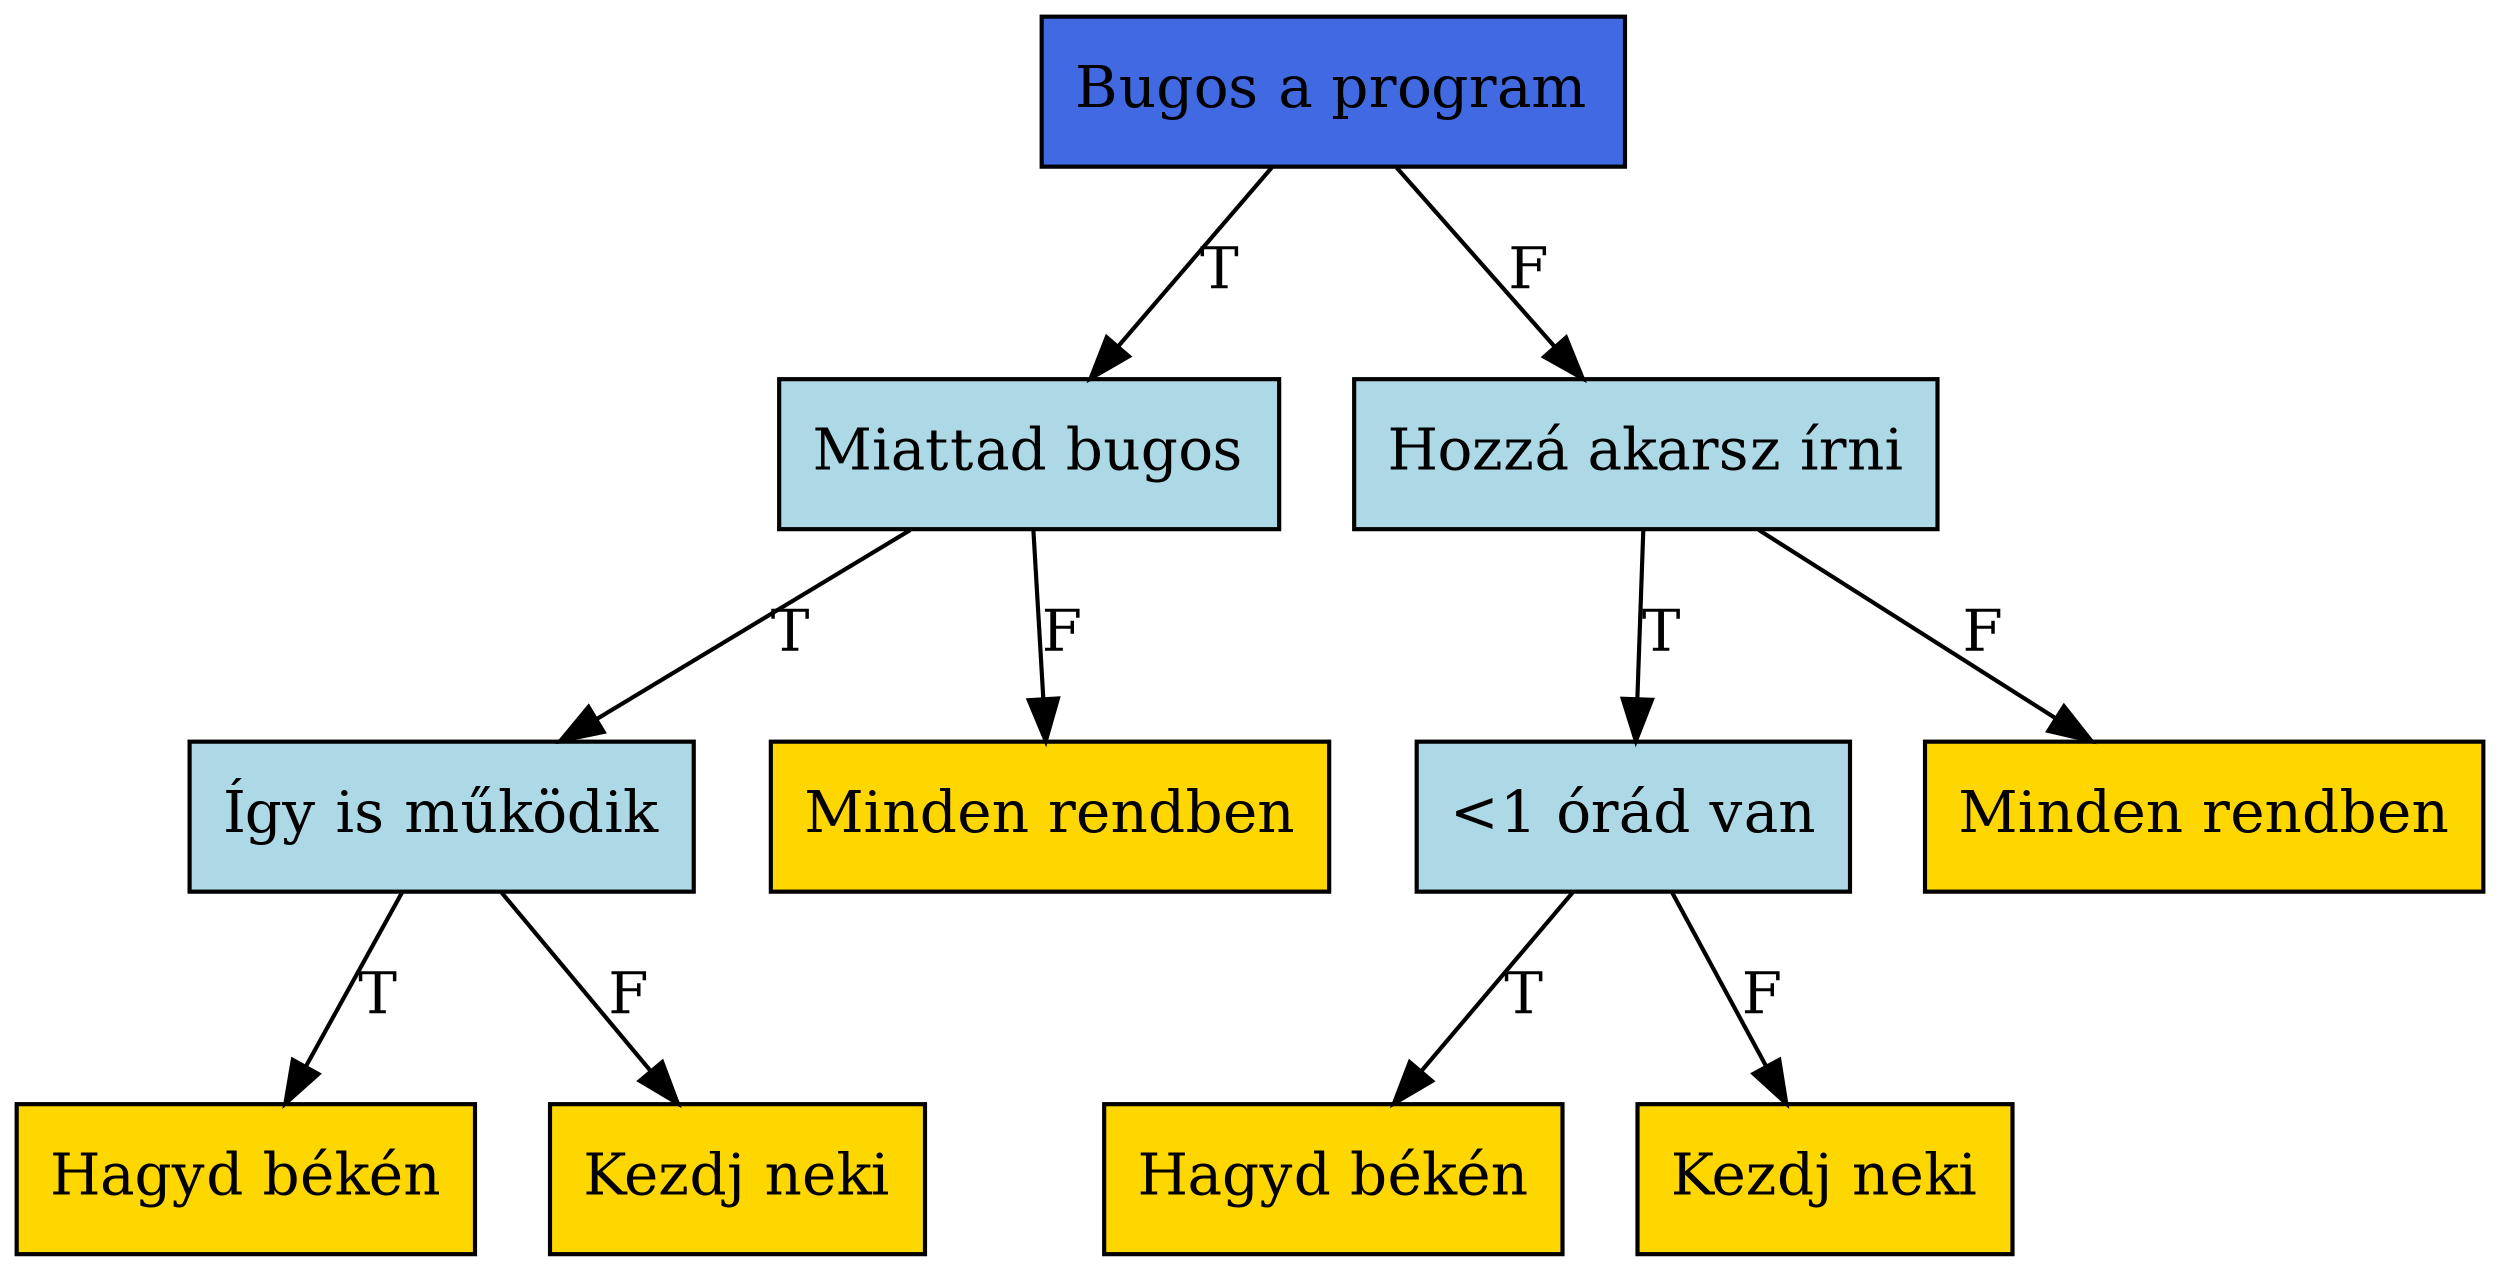
\includegraphics[width=10cm, height=7cm, keepaspectratio]{graphs/decision_trees_2.png}
\end{center}
\end{column}
\end{columns}
\end{frame}

\begin{frame}{A döntési fa komponensei}
\begin{columns}
\begin{column}{.3\textwidth}
\begin{block}{Gyökér csomópont}
Csak outputja van.
\end{block}
\smallskip
\begin{block}{Internális csomópont}
Van inputja és outputja is.
\end{block}
\smallskip
\begin{block}{Levél csomópont}
Csak inputja van.
\end{block}
\end{column}
\begin{column}{.7\textwidth}
\begin{center}
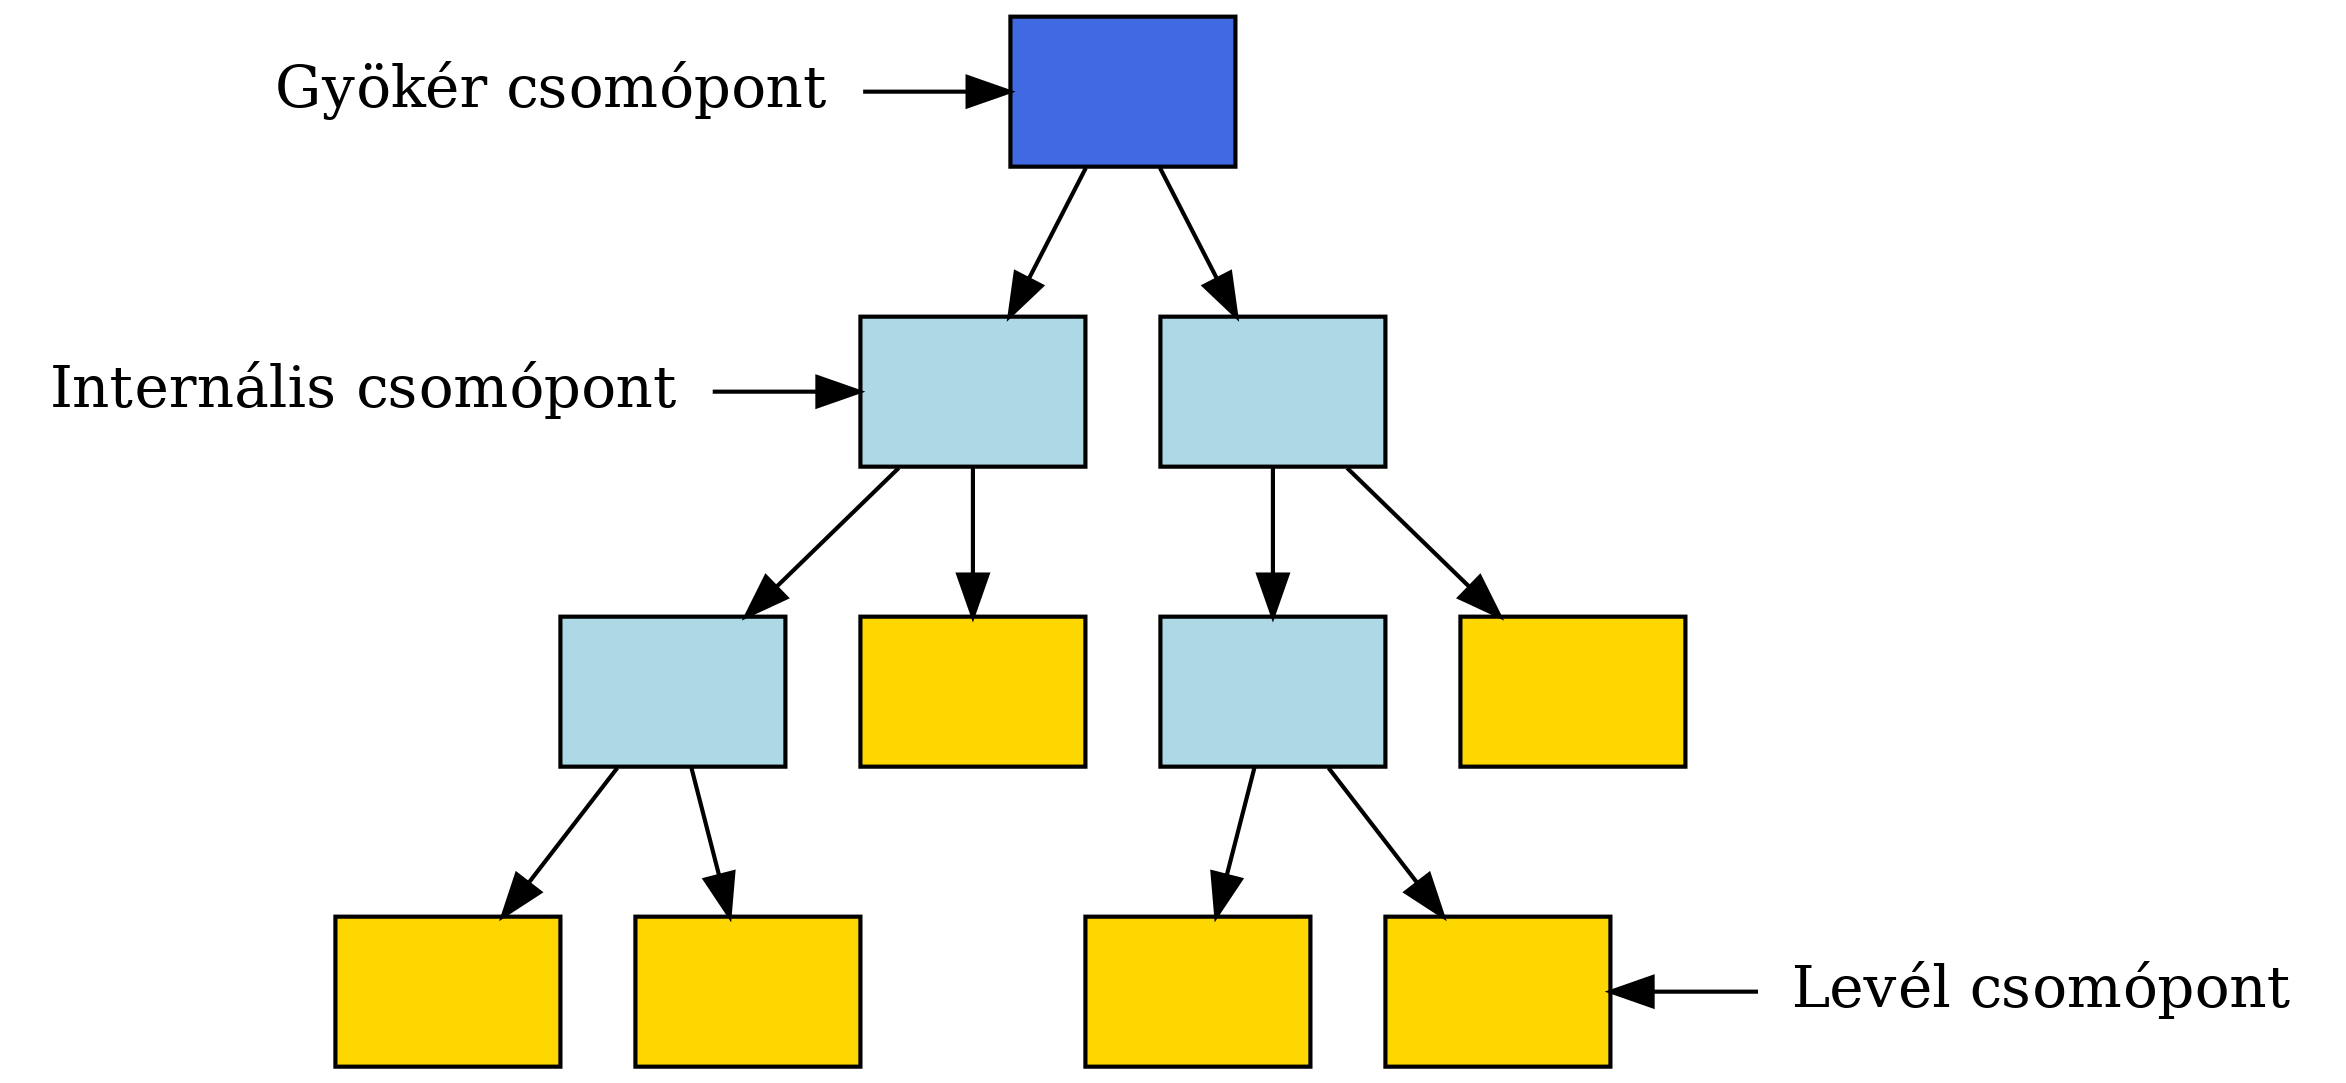
\includegraphics[width=10cm, height=7cm, keepaspectratio]{graphs/decision_trees_3.png}
\end{center}
\end{column}
\end{columns}
\end{frame}

\begin{frame}{Döntési fa az Írisz adathalmazon}
\begin{columns}
\begin{column}{.5\textwidth}
Az első szeparálási változó szirom hossz, aminek a küszöbértéke 2.45 cm. Ha az adott virág szirom hossza kevesebb mint ez az érték akkor a modell szerint a becsült osztály Setosa.\par\smallskip
Ha viszont nagyobb akkor a következő szeparálási ponthoz ér az osztályozás, ami szerint a következő kérdés, hogy a szirom szélesség kisebb-e mint 1.75 cm. Ha igen, a becsült osztály versicolor, egyébként pedig Virginica.
\end{column}
\begin{column}{.5\textwidth}
\begin{center}
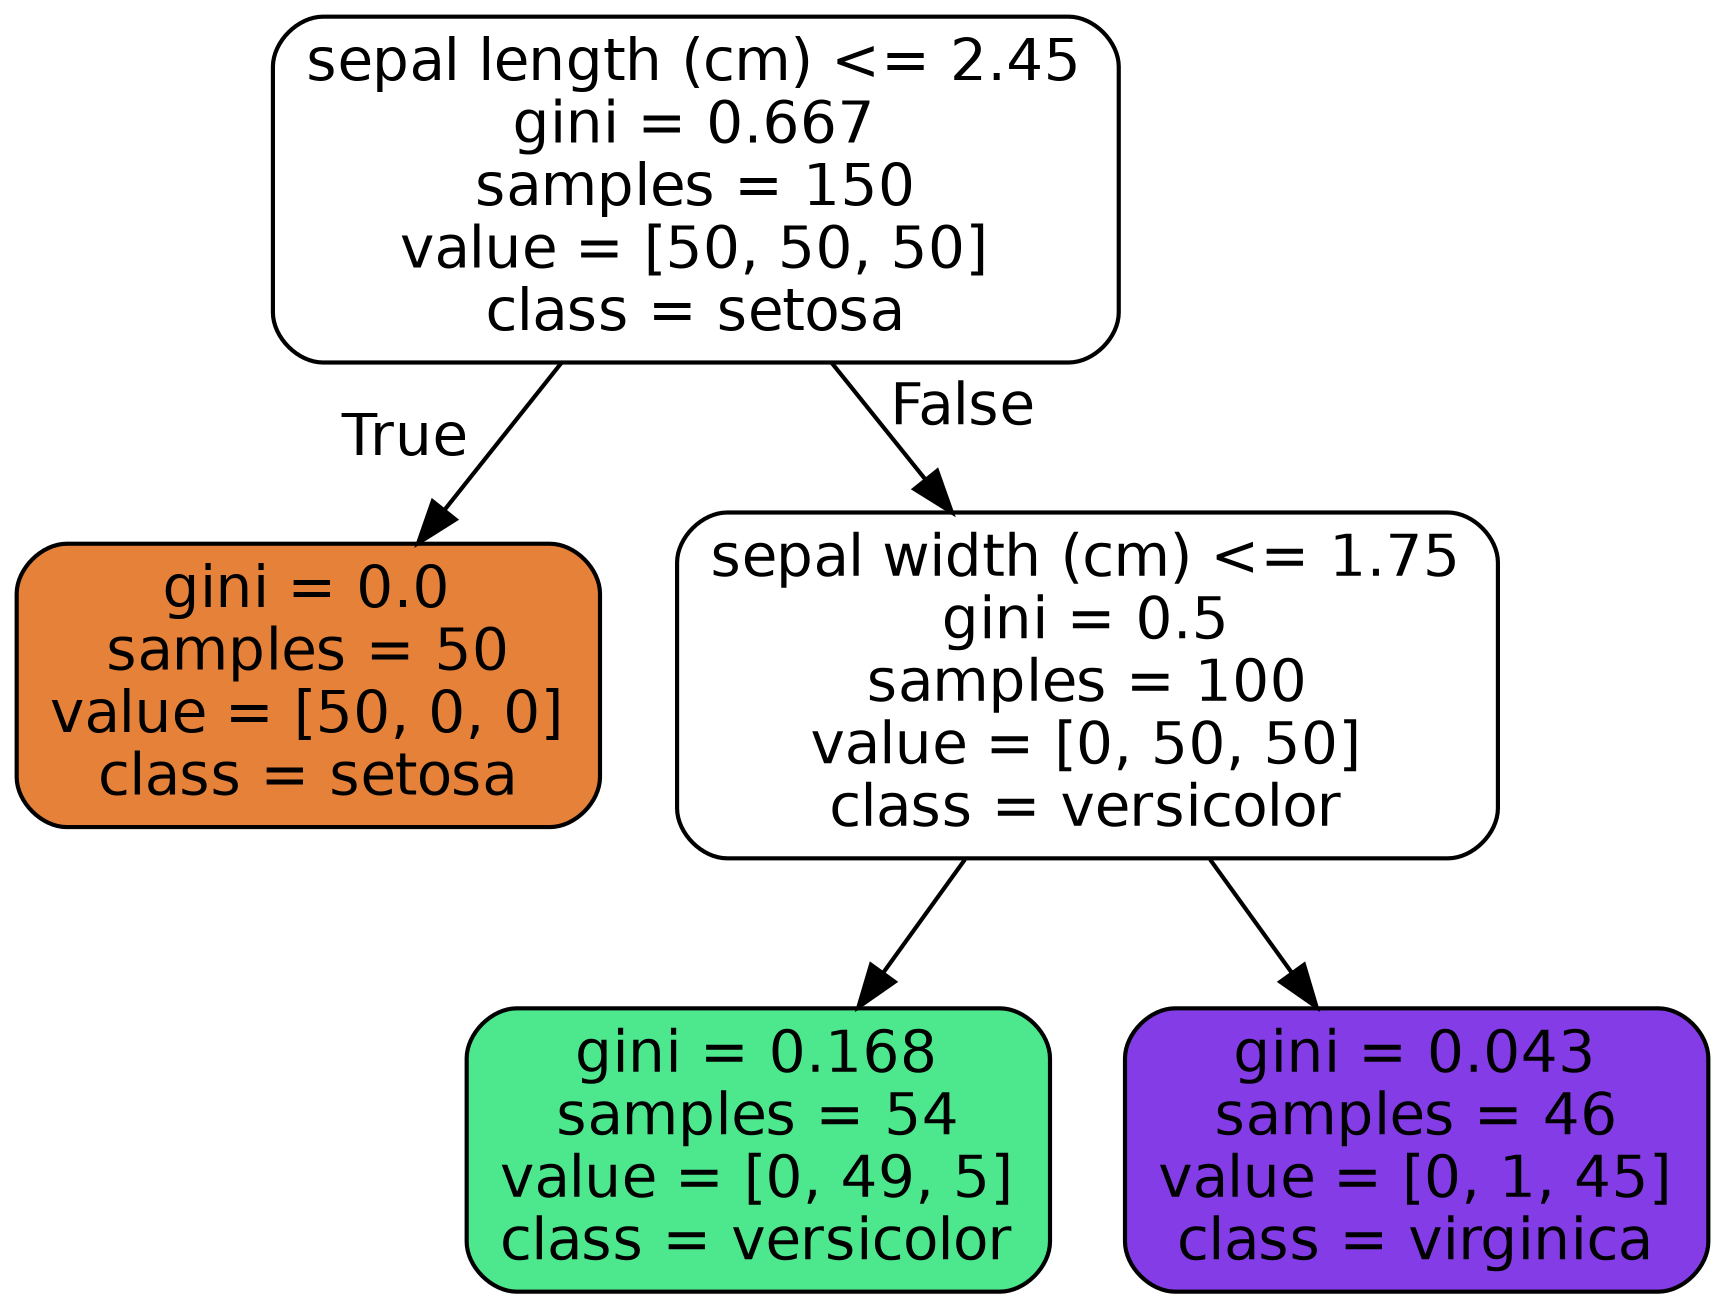
\includegraphics[width=7cm, height=7cm, keepaspectratio]{graphs/decision_trees_4.png}
\end{center}
\end{column}
\end{columns}
\end{frame}

\begin{frame}{A fa ábrázolása}
\begin{columns}
\begin{column}{.4\textwidth}
\begin{center}
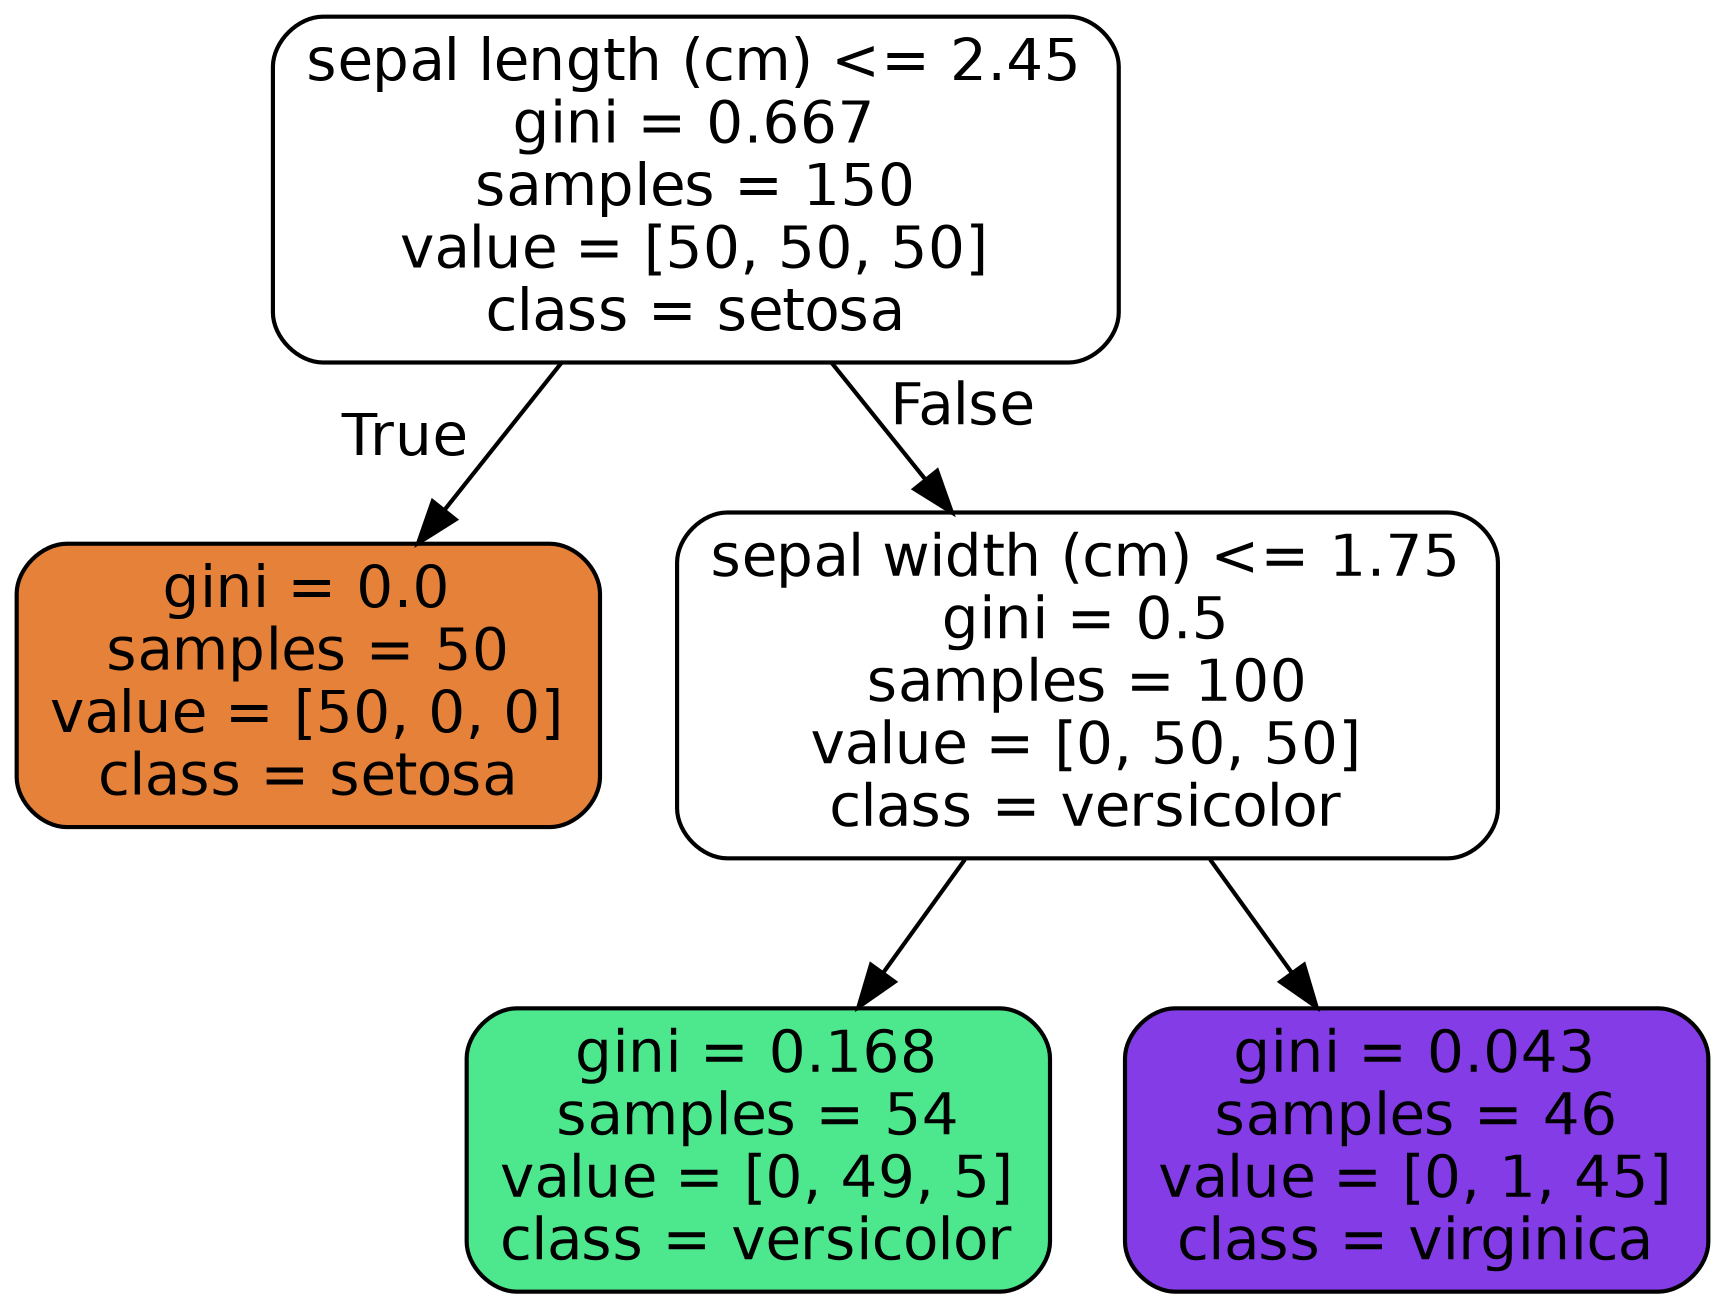
\includegraphics[width=5.5cm, height=7cm, keepaspectratio]{graphs/decision_trees_4.png}
\end{center}
\end{column}
\begin{column}{.6\textwidth}
\begin{center}
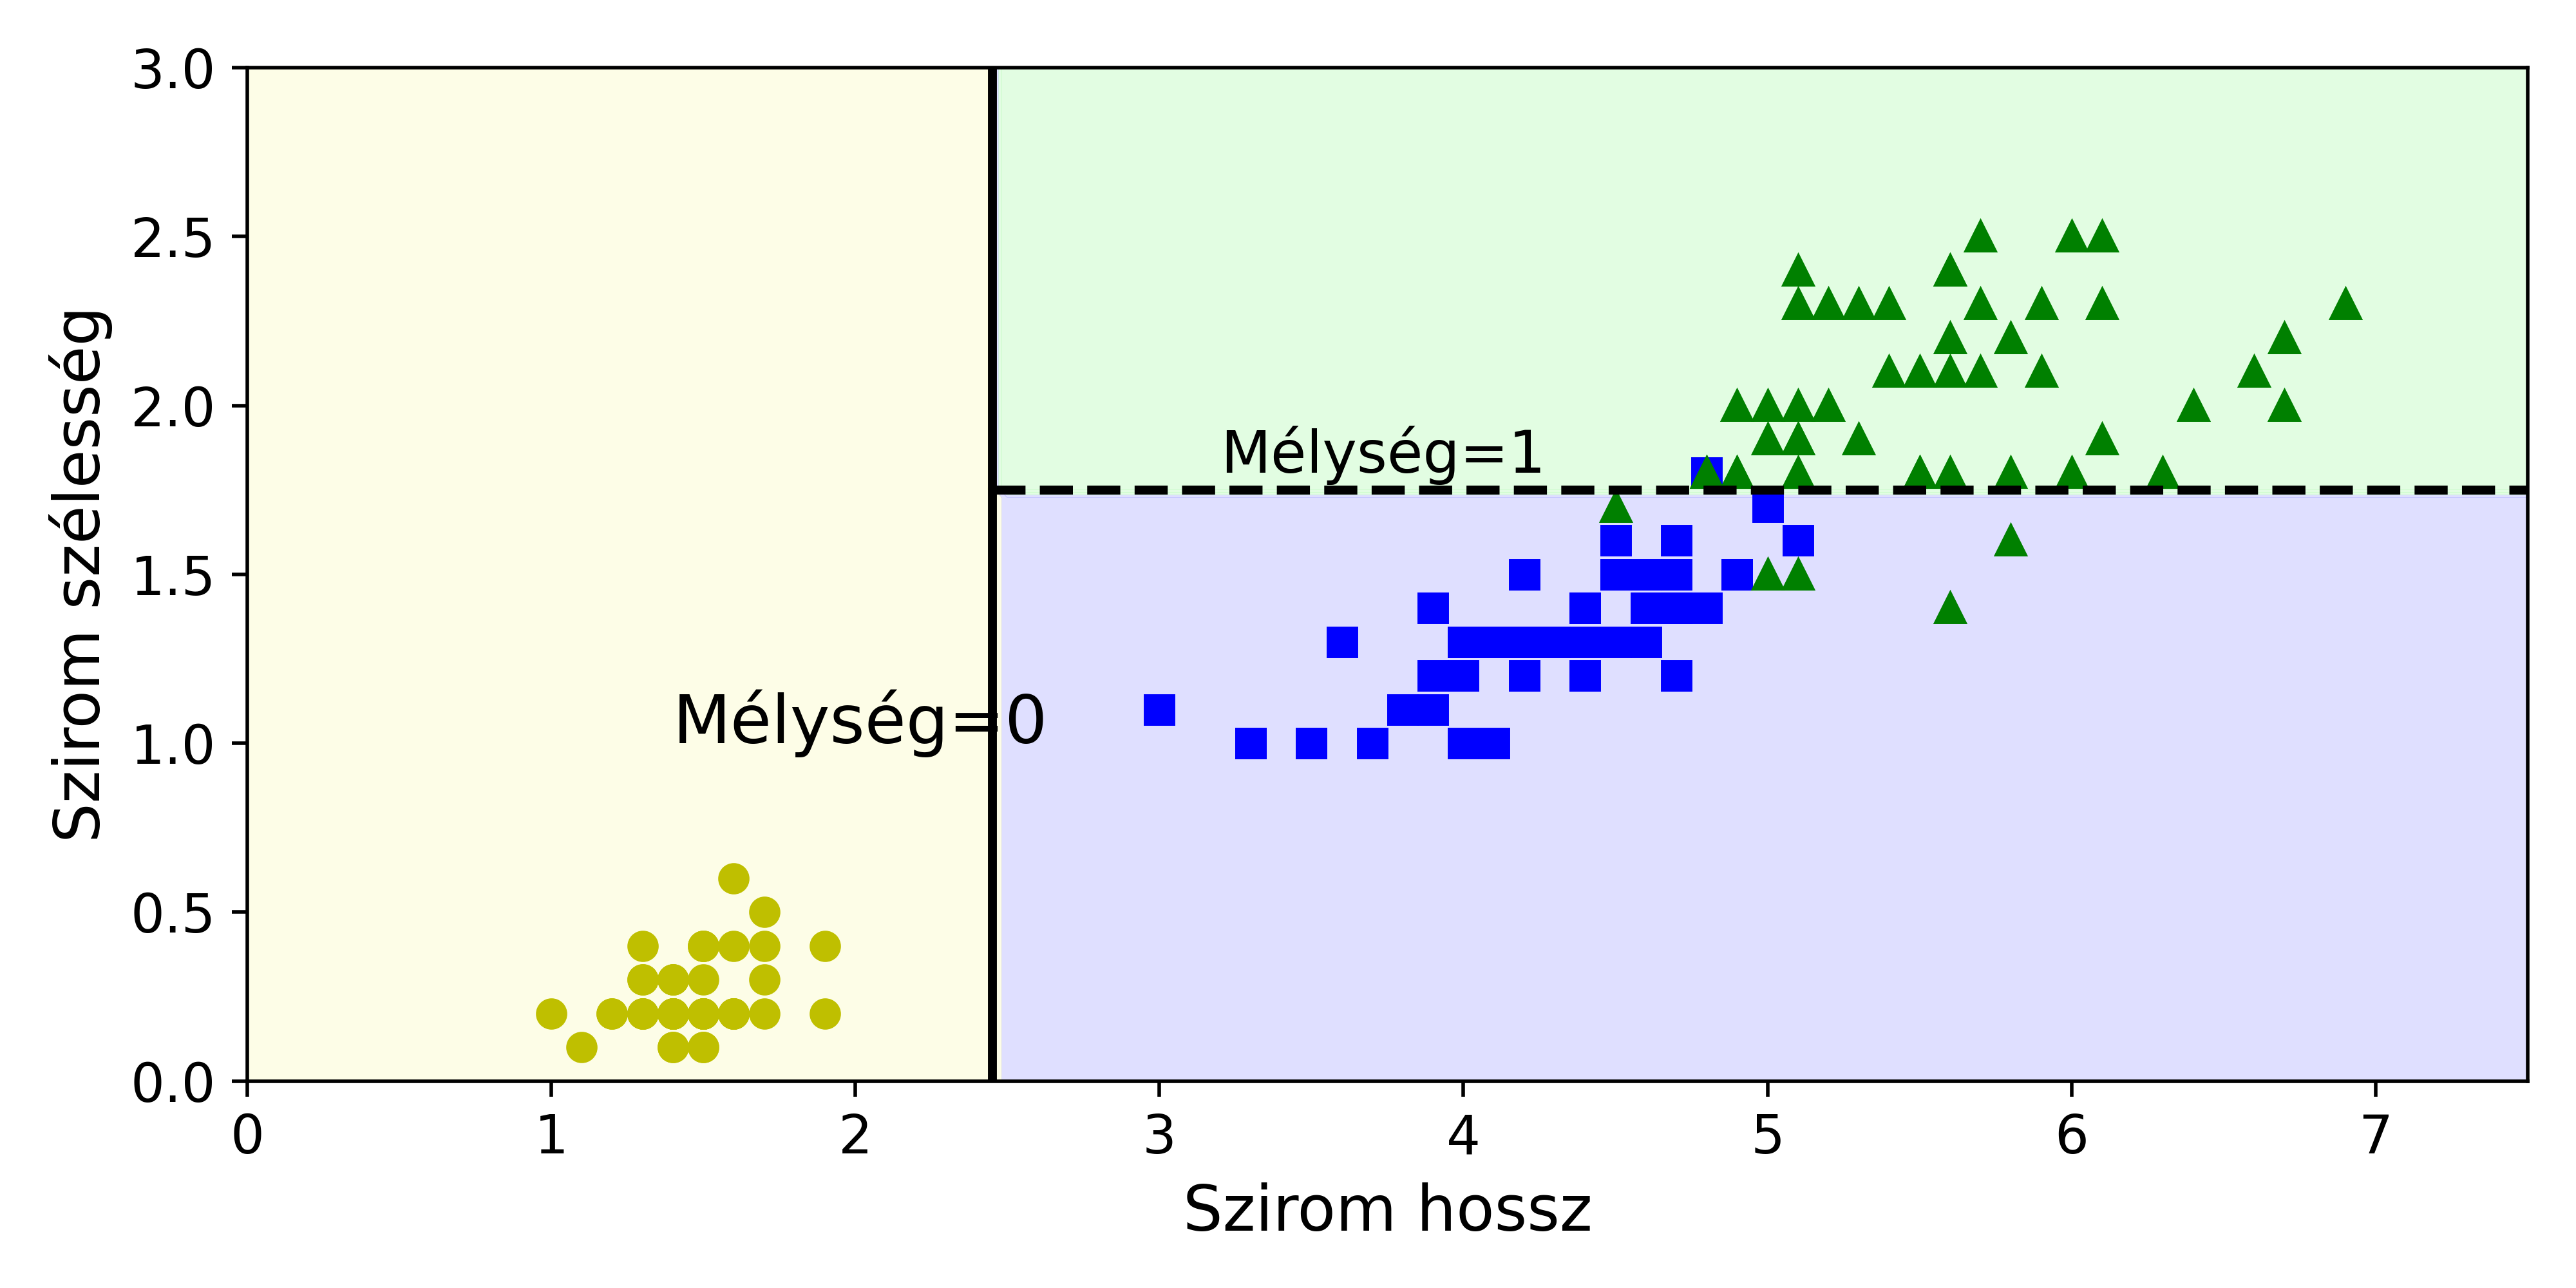
\includegraphics[width=8cm, height=7cm, keepaspectratio]{images/decision_trees_2.png}
\end{center}
\end{column}
\end{columns}
\vspace{0.5cm}
A vastag vonal a gyökérből származó határ. Mivel a bal oldali halmaz teljesen tiszta, nem lehet tovább bontani. De a jobb oldali részhalmaz továbbra is kevert, ezért a jobb oldali első szintű belső nódus tovább bontja 1.75cm küszöbnél.
\end{frame}

\section{Tanítás}

\begin{frame}
\tableofcontents[currentsection]
\end{frame}

\begin{frame}{Tisztátalanság}
\begin{columns}
\begin{column}{.4\textwidth}
Azok a változók, amelyek nem képesek $1:0$ arányban szeparálni az egyedeket tisztátalannak számítanak. Ennek egyik mutatószáma a Gini-index.
\begin{block}{Gini}
\vspace{-.2cm}
\[
G\left( x \right) = 1 - P\left(A\right)^2 - P\left(B\right)^2 
\]
\vspace{-.5cm}
\begin{itemize}
	\item $P\left(\cdot\right)$: adott levélbe kerülés valószínűsége
\end{itemize}
Egy változó Gini-indexe leveleinek Gini-indexeinek súlyozott átlaga.
\end{block}
\end{column}
\begin{column}{.6\textwidth}
\begin{center}
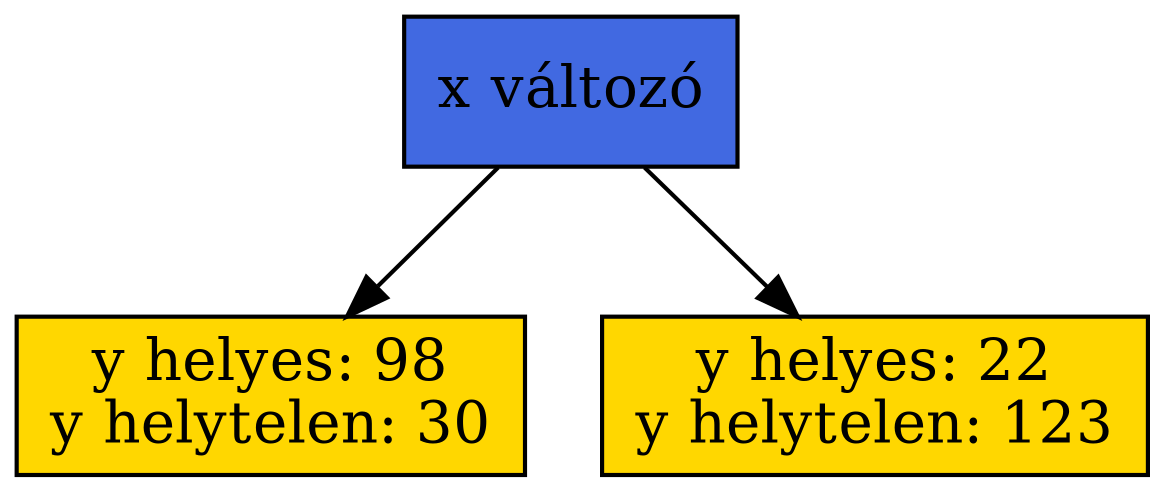
\includegraphics[width=7cm, height=7cm, keepaspectratio]{graphs/decision_trees_5.png}
\end{center}
\[
G\left(A\right) = 1 - \left(\frac{98}{98 + 30}\right)^2 - \left(\frac{30}{98 + 30}\right)^2 = 0.35
\]
\[
G\left(B\right) = 1 - \left(\frac{22}{22 + 123}\right)^2 - \left(\frac{123}{22 + 123}\right)^2 = 0.25
\]
\[
G\left(x\right) = \left( \frac{128}{128 + 145} \right)0.35 + \left( \frac{145}{128 + 145} \right) 0.25 = 0.3
\]
\end{column}
\end{columns}
\end{frame}

\begin{frame}{Szeparáció folytonos változó esetén}
\begin{columns}
\begin{column}{.5\textwidth}
\only<1>{A folytonos változónak minden értékéhez tartozik egy Gini-index.\par\medskip
Egy adott $x$ változóra a $t_x$ küszöbérték menti szeparáció, hogy az egyik partícióba azon mintaegyedek kerülnek, amelyekre $x \leq t_x$ a másikba pedig amelyekre $x > t_x$.}
\only<2>{Ennek megfelelően a szeparáció ott a legjobb, ahol a $G(t_x)$ függvénynek minimuma van.}
\end{column}
\begin{column}{.5\textwidth}
\begin{center}
\includegraphics<1>[width=7cm, height=7cm, keepaspectratio]{graphs/decision_trees_6.png}
\includegraphics<2>[width=7cm, height=7cm, keepaspectratio]{images/decision_trees_3.png}
\end{center}
\end{column}
\end{columns}
\end{frame}

\begin{frame}{Mikor érdemes szeparálni?}
\begin{columns}
\begin{column}{.5\textwidth}
Amikor egy csomópontnak \textbf{magasabb a tisztátalansága tovább bontáskor}, felesleges a szeparáció és levélcsomópont válik belőle.\par\medskip
Gyökércsomópont abból a változóból válik, amelynek \textbf{a legalacsonyabb a tisztátalansága}.\par\medskip
\only<1>{Ebben az esetben szeparációval $G=0.29$}
\only<2>{Szeparáció nélkül $G=0.20$, tehát \textbf{a szeparáció felesleges}.}
\end{column}
\begin{column}{.5\textwidth}
\begin{center}
\includegraphics<1>[width=7cm, height=7cm, keepaspectratio]{graphs/decision_trees_7.png}
\includegraphics<2>[width=7cm, height=7cm, keepaspectratio]{graphs/decision_trees_8.png}
\end{center}
\end{column}
\end{columns}
\end{frame}

\begin{frame}{A CART tanító algoritmus}
\begin{columns}
\begin{column}{.5\textwidth}
A \textbf{C}lassification \textbf{A}nd \textbf{R}egression \textbf{T}rees egy döntési fák tanítására használt algoritmus.\par\smallskip
Az eljárás $x$ változóra és $t_x$ küszöbértékre olyan $\left(x,t_x\right)$ párokat keres, amelyekre a létrejövő részhalmazoknak a lehető legalacsonyabb a tisztátalansága.\par\smallskip
Ezt rekurzívan ismétli kilépésig.
\end{column}
\begin{column}{.5\textwidth}
\begin{block}{A CART költségfüggvénye}
\[
J\left(x,t_x\right) = \frac{m_{A}}{m}G_A + \frac{m_B}{m}G_B
\]
Ahol:
\begin{itemize}
	\item $G_A$: Bal oldali nódus Gini-indexe
	\item $G_B$: Jobb oldali nódus Gini-indexe
	\item $m_A$: Bal oldali nódusba bekerült egyedek száma
	\item $m_B$: Jobb oldali nódusba bekerült egyedek száma
	\item $m$: Egyedek száma a teljes halmazban
\end{itemize}
\end{block}
\end{column}
\end{columns}
\end{frame}

\begin{frame}{Korai leállás döntési fák esetén}
\begin{columns}
\begin{column}{.5\textwidth}
Túltanulás esetén a \textbf{tanító pontosság nagyon magas lesz, viszont a teszt pontosság alacsony}.\par\smallskip
Döntési fák esetén annyi változót érdemes meghagyni a modellezés során, amennyivel a lehető legmagasabb a teszt pontosság.\par\smallskip
Korai leállás esetén \textbf{a modell kiszáll a tanításból, ha a validációs pontosság elkezd csökkenni}. 
\end{column}
\begin{column}{.5\textwidth}
\begin{center}
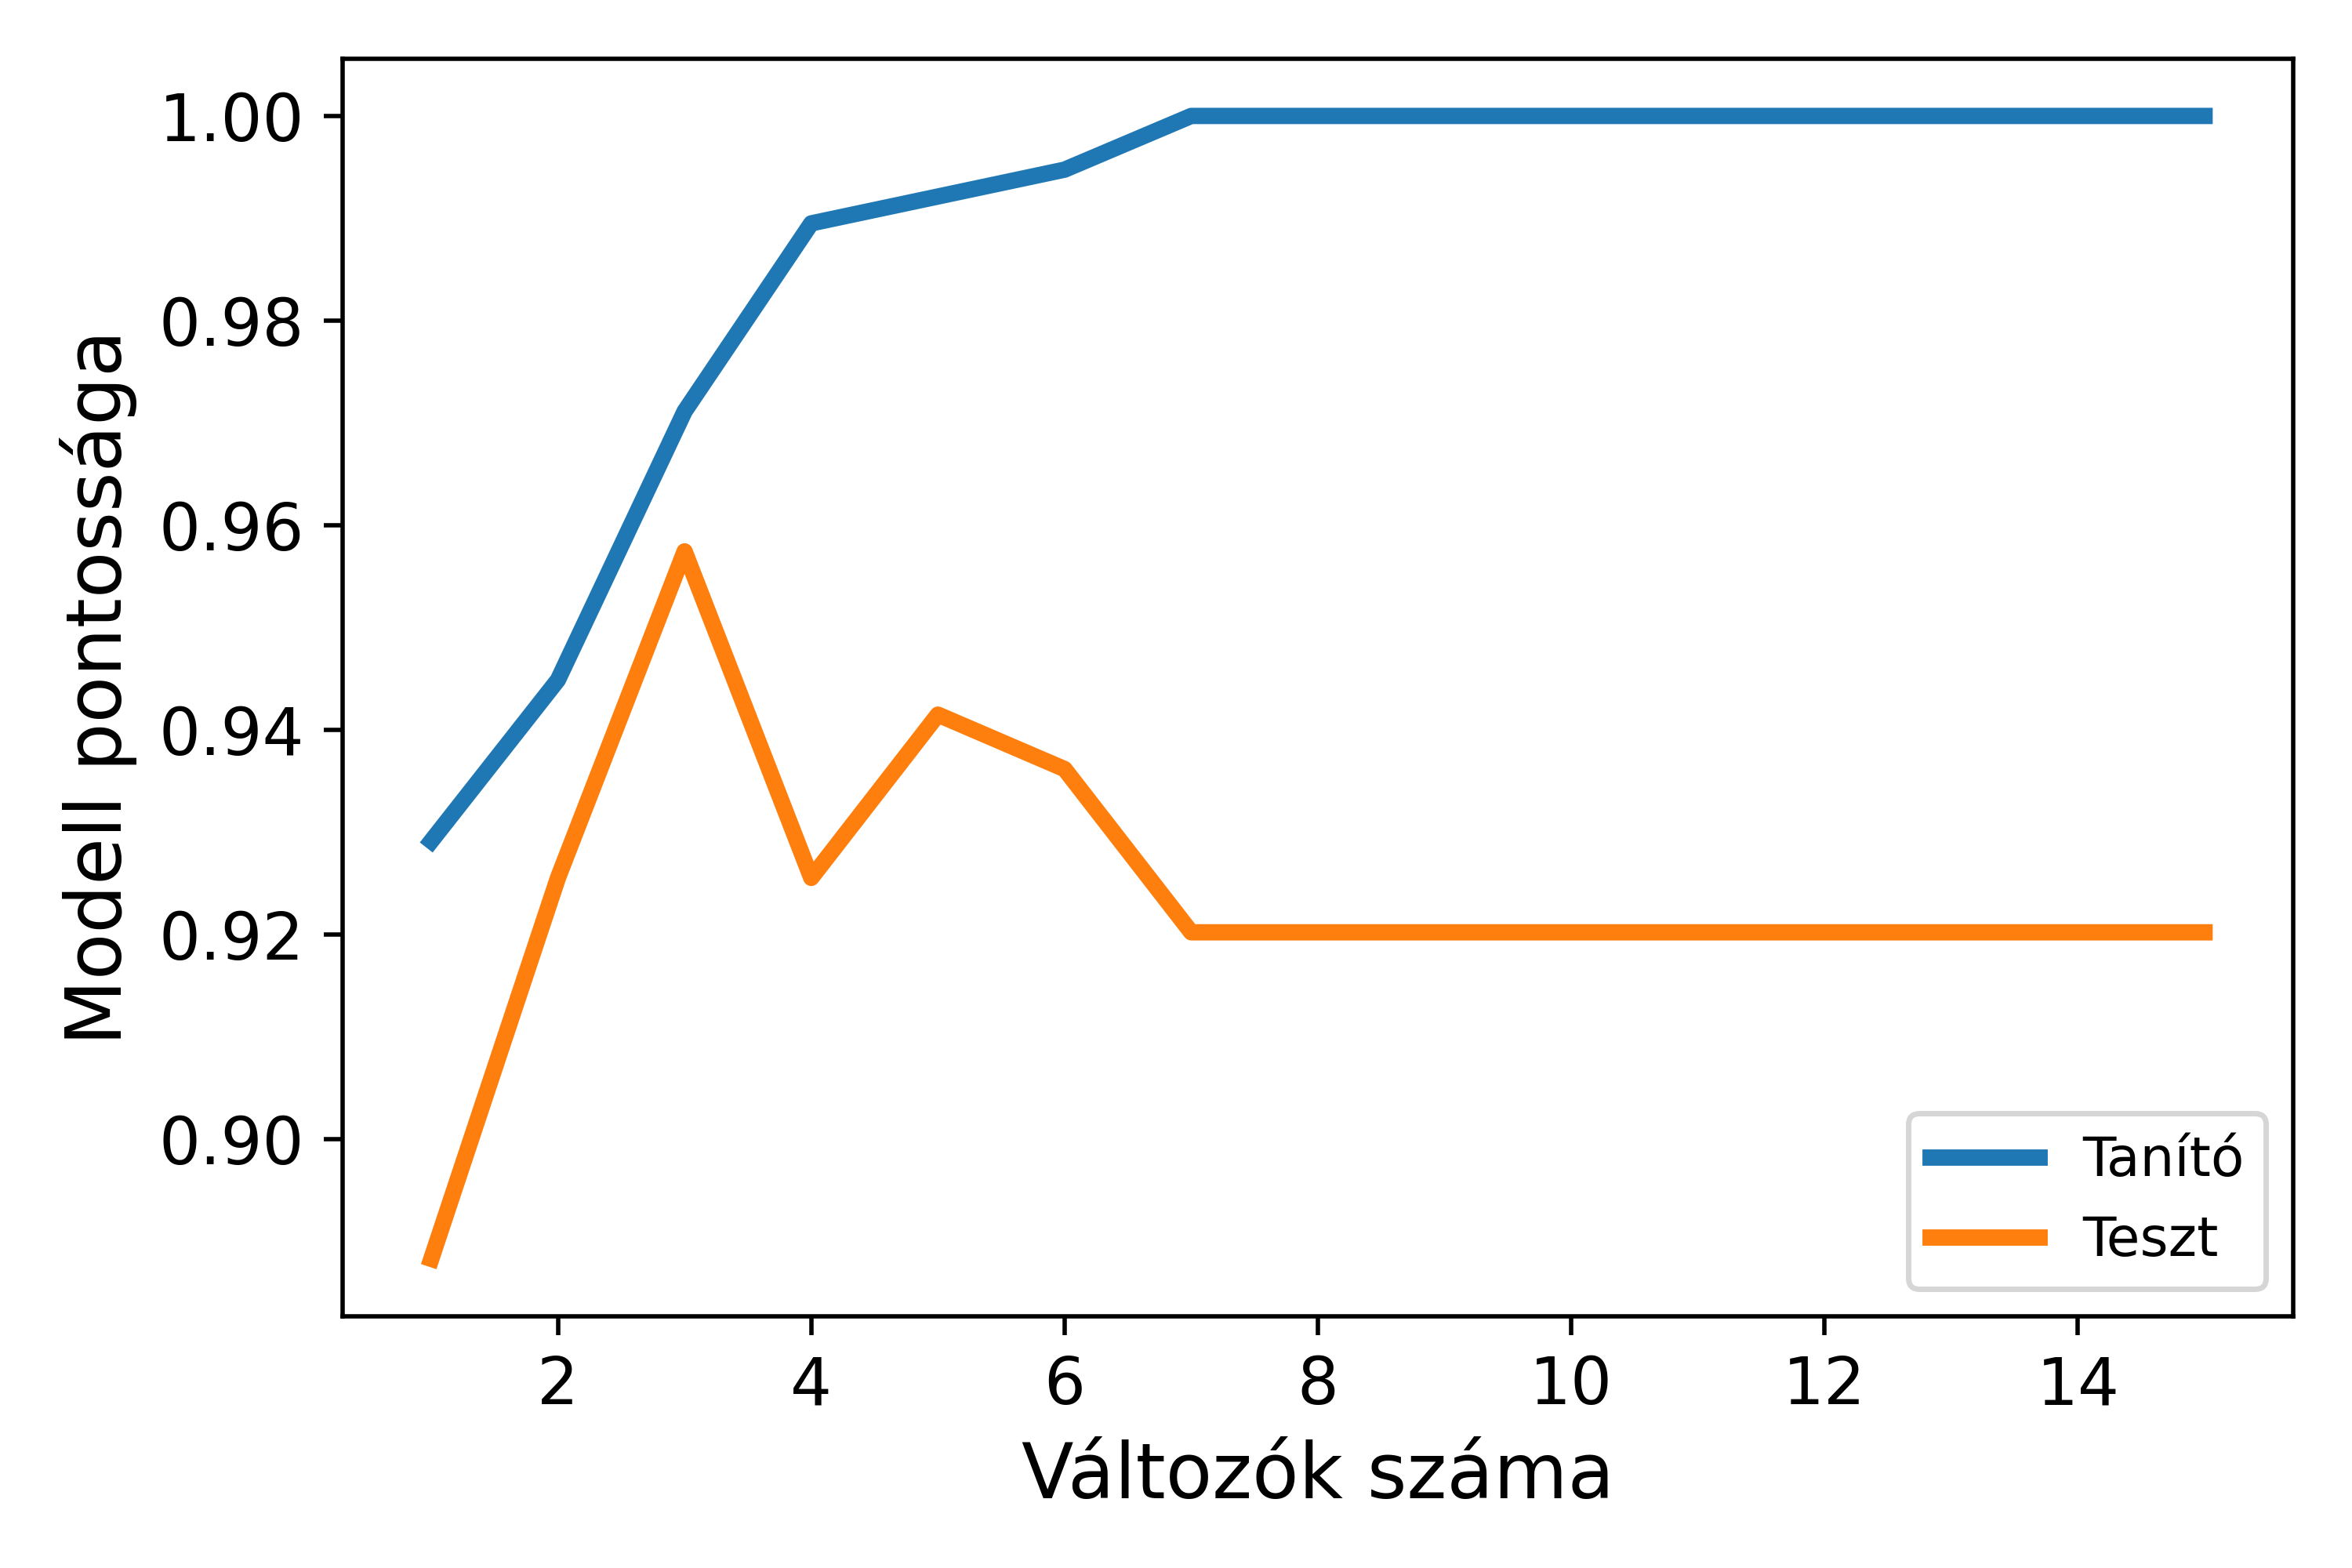
\includegraphics[width=7cm, height=7cm, keepaspectratio]{images/decision_trees_5.png}
\end{center}
\end{column}
\end{columns}
\end{frame}

\begin{frame}{Döntési fák regularizálása}
A döntési fák meglehetősen kevés előfeltételezéssel élnek az adathalmaz irányába. Ha megkötések nélkül van tanítva, \textbf{könnyen túltanulhat a modell}.\par\medskip
A bal oldali ábrán egy regularizáció nélküli, a jobb oldalon pedig egy \texttt{min\_samples\_leaf=4} paraméterrel tanított döntési fa látható. 
\begin{center}
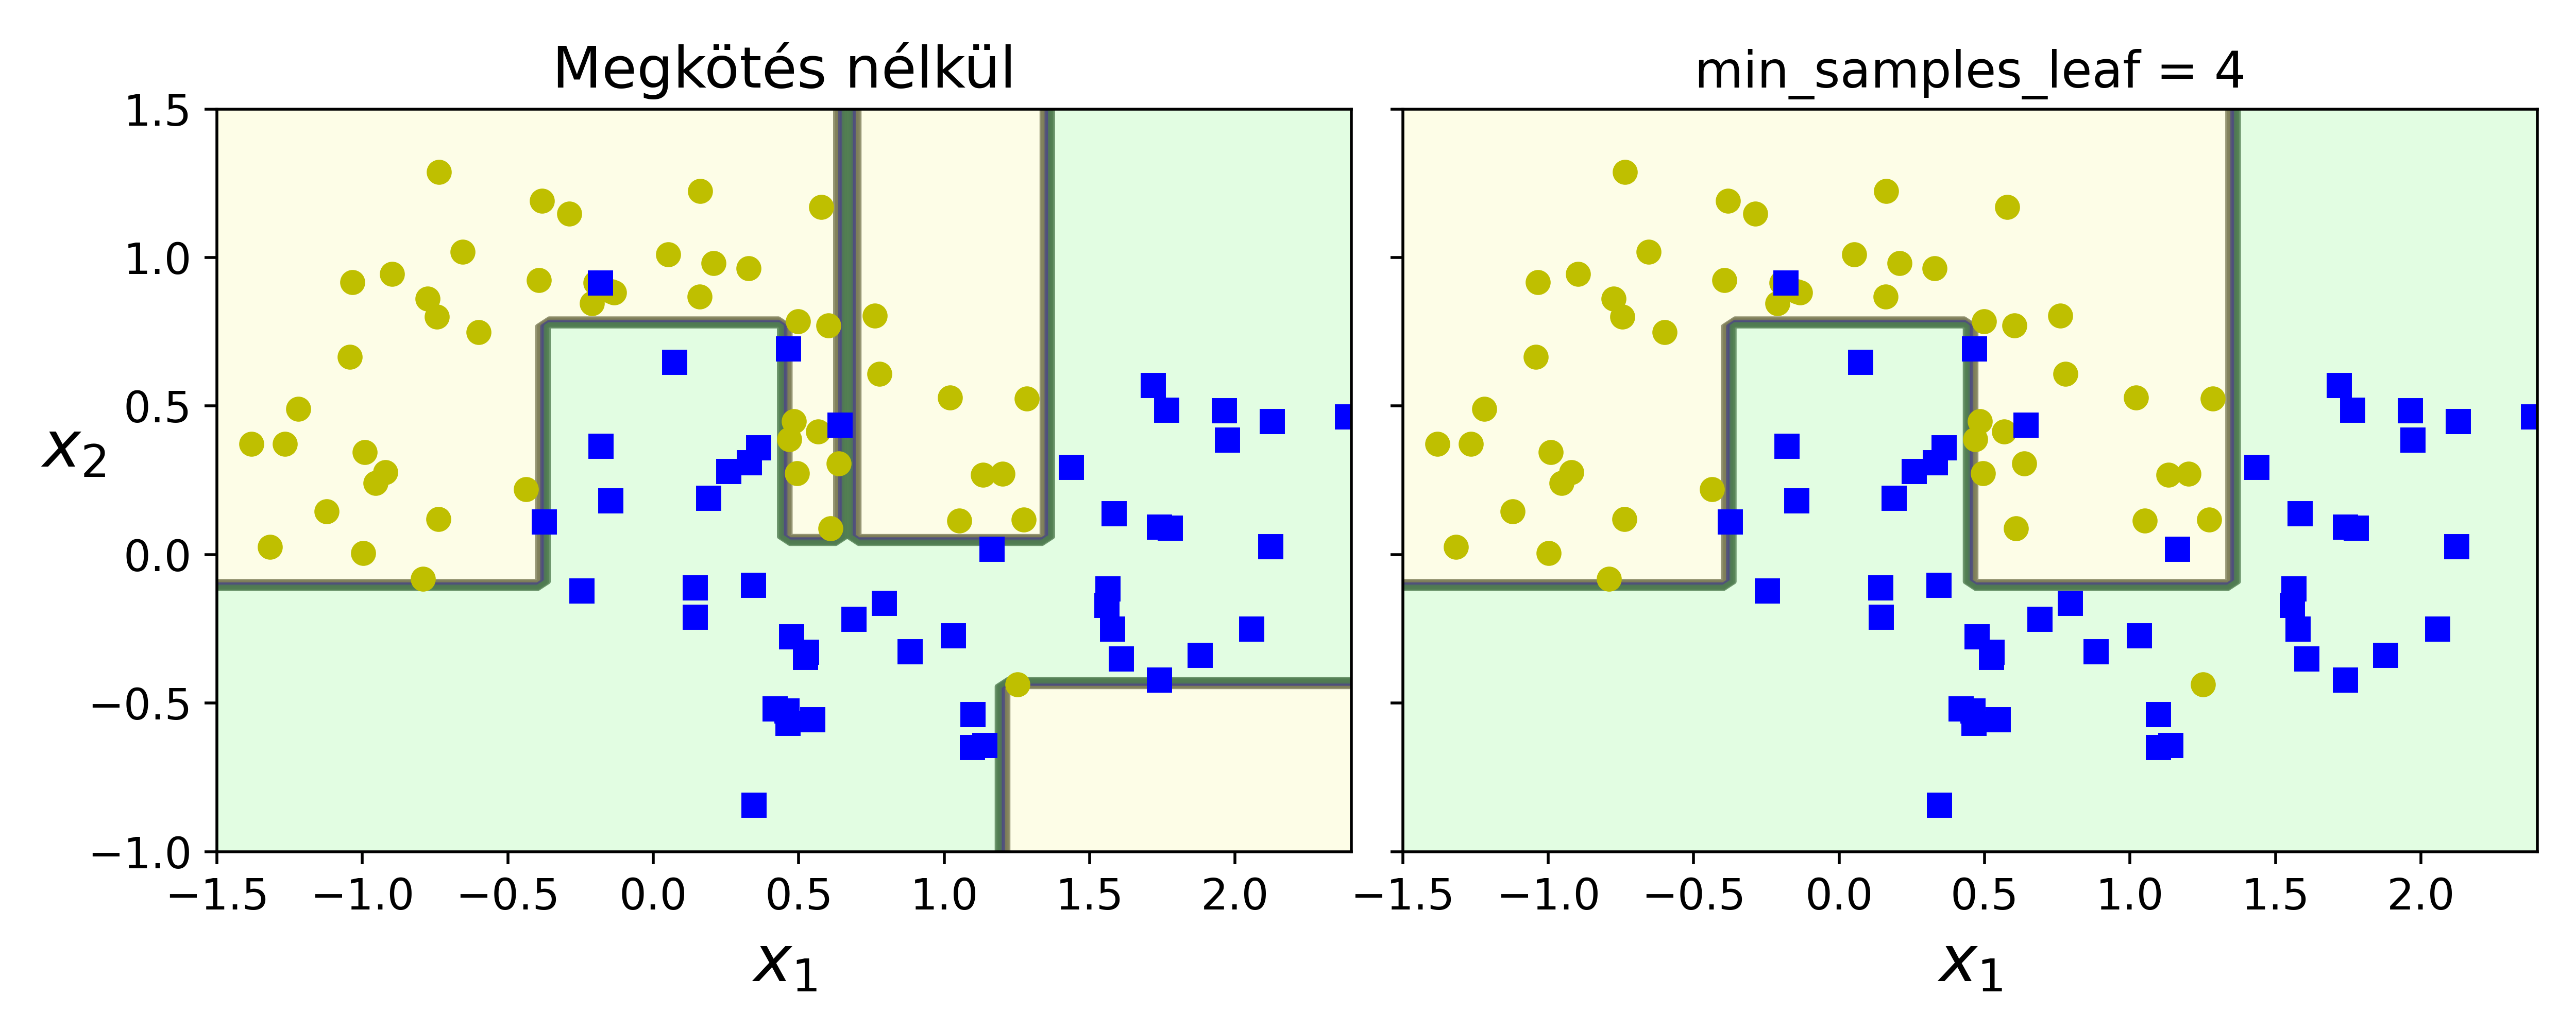
\includegraphics[width=12cm, height=7cm, keepaspectratio]{images/decision_trees_4.png}
\end{center}
\end{frame}

\begin{frame}{Regresszió döntési fákkal}
Regresszió esetén a döntési fák leveleikben folytonos változókhoz tartozó értékékeket vesznek fel. Ebben az esetben a predikció a levelekbe bekerült mintaegyedek célváltozóikban felvett értékeinek az átlaga. 
\begin{center}
\includegraphics<1>[width=12cm, height=7cm, keepaspectratio]{graphs/decision_trees_9.png}
\includegraphics<2>[width=12cm, height=7cm, keepaspectratio]{images/decision_trees_6.png}
\end{center}
\end{frame}

\begin{frame}{Regularizáció regresszor fák esetén}
Az osztályozó fákhoz hasonlóan a regresszor fák is hajlamosak a túltanulásra. A regularizáció olyan paraméterek állításával érhető el, mint a \texttt{min\_samples\_leaf}, \texttt{min\_samples\_split}, \texttt{max\_leaf\_nodes}, \texttt{max\_depth}.
\begin{center}
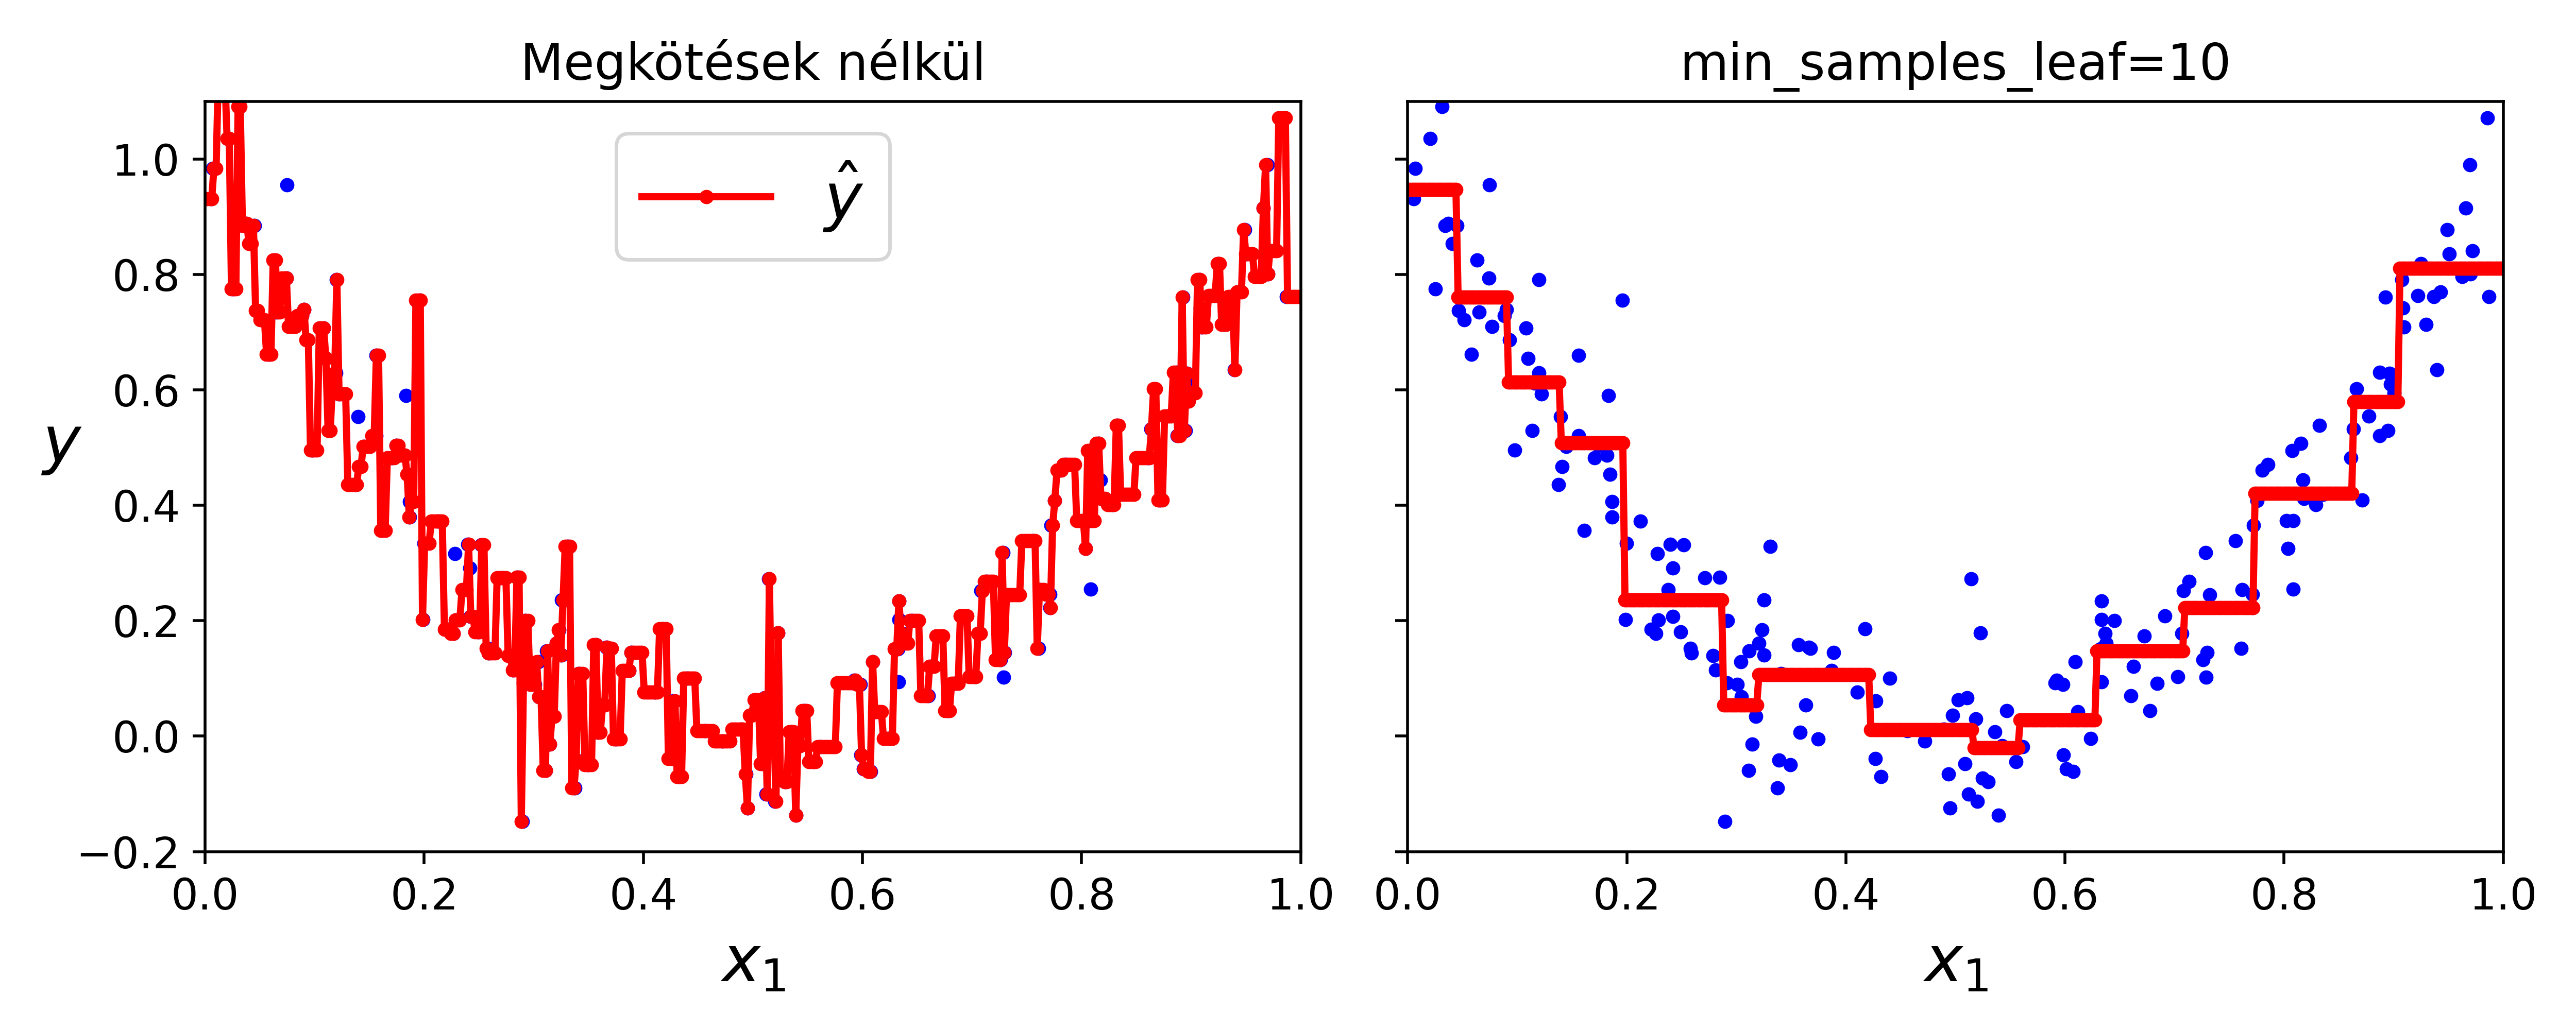
\includegraphics[width=12cm, height=7cm, keepaspectratio]{images/decision_trees_7.png}
\end{center}
\end{frame}

\begin{frame}{CART tanító algoritmus regressziós fákra}
\begin{columns}
\begin{column}{.5\textwidth}
A regresszor fák a tisztátalanság helyett az MSE metrikát minimalizálják.\par\medskip
\begin{block}{Csomópont becsült értéke}
Egy $A$ nódus becsült értéke a bele került mintaegyedek célváltozóikban felvett értékeinek átlaga: 
\[
\hat{y}_A = \frac{1}{m_A}\sum_{i \in m_A} y_i
\]
\end{block}
\end{column}
\begin{column}{.5\textwidth}
\begin{block}{A CART regresszor algoritmus költségfüggvénye}
\[
J\left( x,t_x \right) = \frac{m_A}{m}MSE_A + \frac{m_B}{m}MSE_B
\]
Ahol:
\begin{itemize}
	\item $MSE_A = \sum_{i \in m_A} \left( \hat{y} - y_i \right)^2$: $A$ csomópont átlagos négyzetes hibája
	\item $MSE_B = \sum_{i \in m_B} \left( \hat{y} - y_i \right)^2$: $B$ csomópont átlagos négyzetes hibája
\end{itemize}
\end{block}
\end{column}
\end{columns}
\end{frame}

\section{Döntési fák tulajdonságai}

\begin{frame}
\tableofcontents[currentsection]
\end{frame}

\begin{frame}{Instabilitás: rotáció az adathalmazon}
\only<1>{Az alábbi példában egy lineárisan szeparálható adathalmazon történt $45^\circ$-os forgatás után látható ugyanannak a modellnek a predikciója. A létrejövő döntési határ jóval komplexebb a transzformált adathalmaz esetén.}
\only<2>{Az következő példában az Írisz adathalmazon egy $180^\circ$-os forgatás után láthatóak hasonló módon paraméterezett modellek döntési határai. Érdemes megfigyelni, mennyire különbözik a predikció a torzított adathalmazon.}
\begin{center}
\includegraphics<1>[width=12cm, keepaspectratio]{images/decision_trees_8.png}
\includegraphics<2>[width=7cm, height=7cm, keepaspectratio]{images/decision_trees_9.png}\includegraphics<2>[width=7cm, height=7cm, keepaspectratio]{images/decision_trees_10.png}
\end{center}
\end{frame}

\begin{frame}{Instabilitás: variációk az adathalmazban}
Ebben az esetben a legszélesebb Versicolor (kék) nem került bele a minta adathalmazba. Egyetlen minta adatpont változása is nagy torzítást képes bevinni a modellbe.
\begin{center}
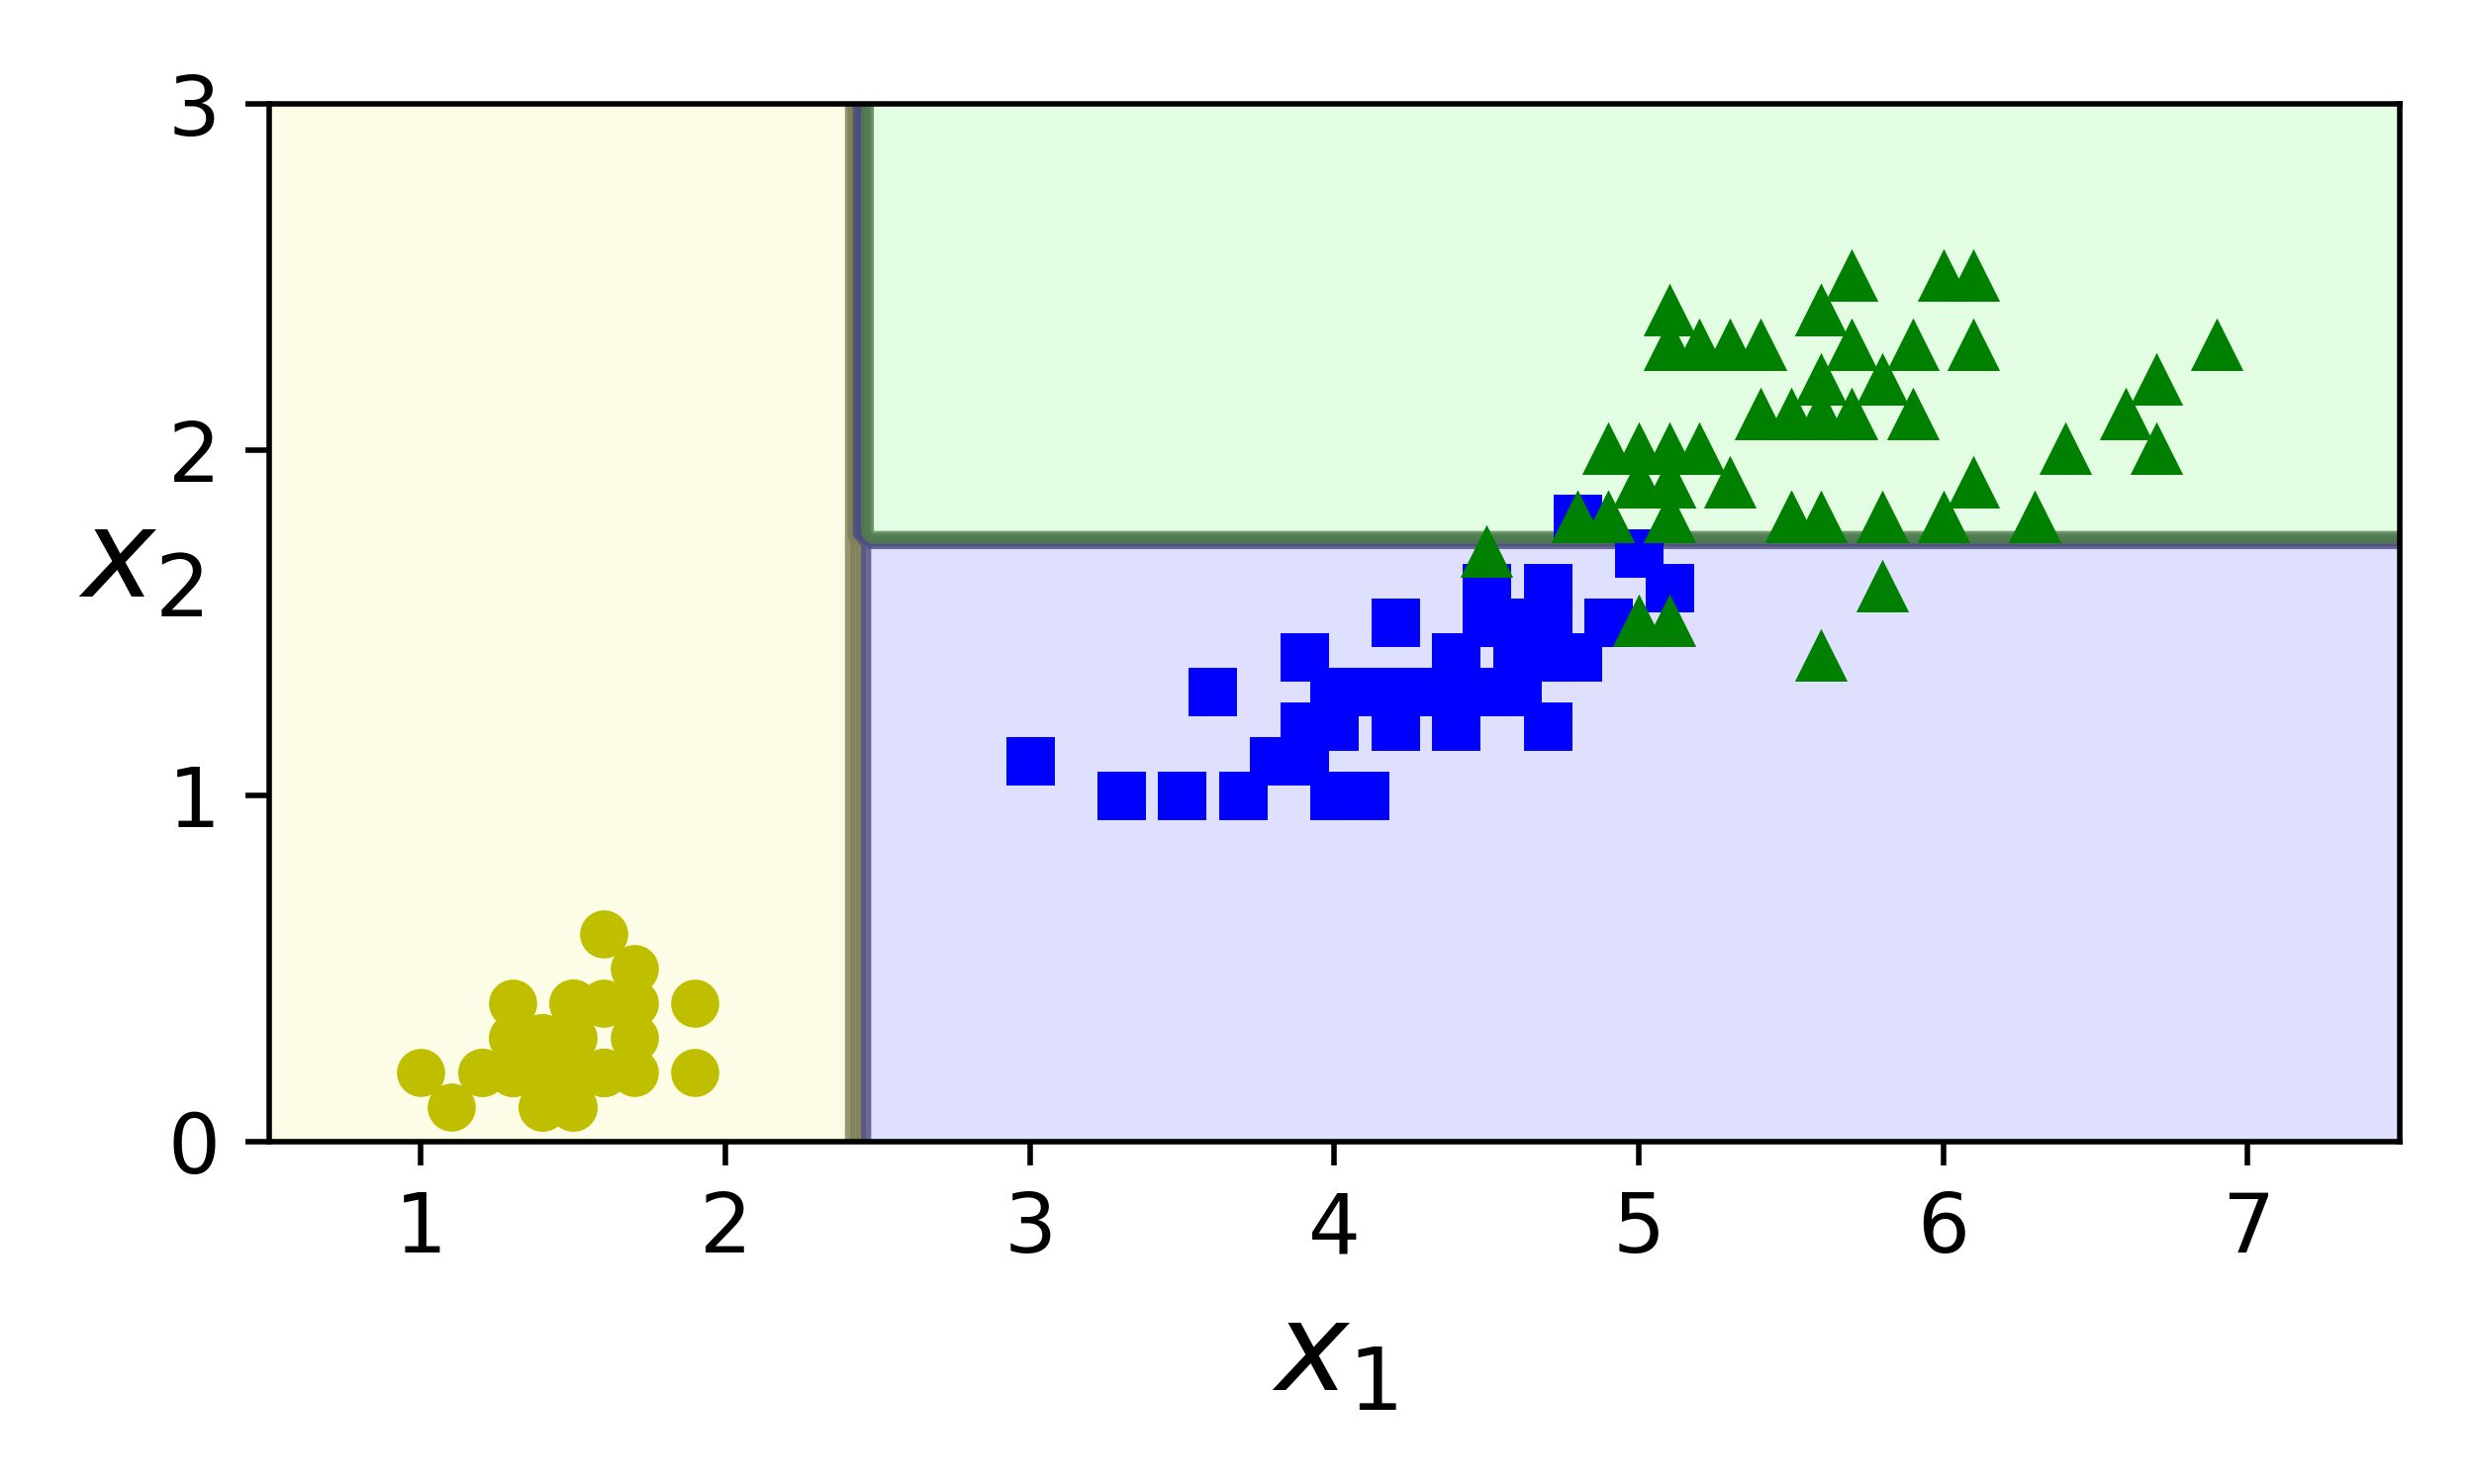
\includegraphics[width=7cm, height=7cm, keepaspectratio]{images/decision_trees_9.png}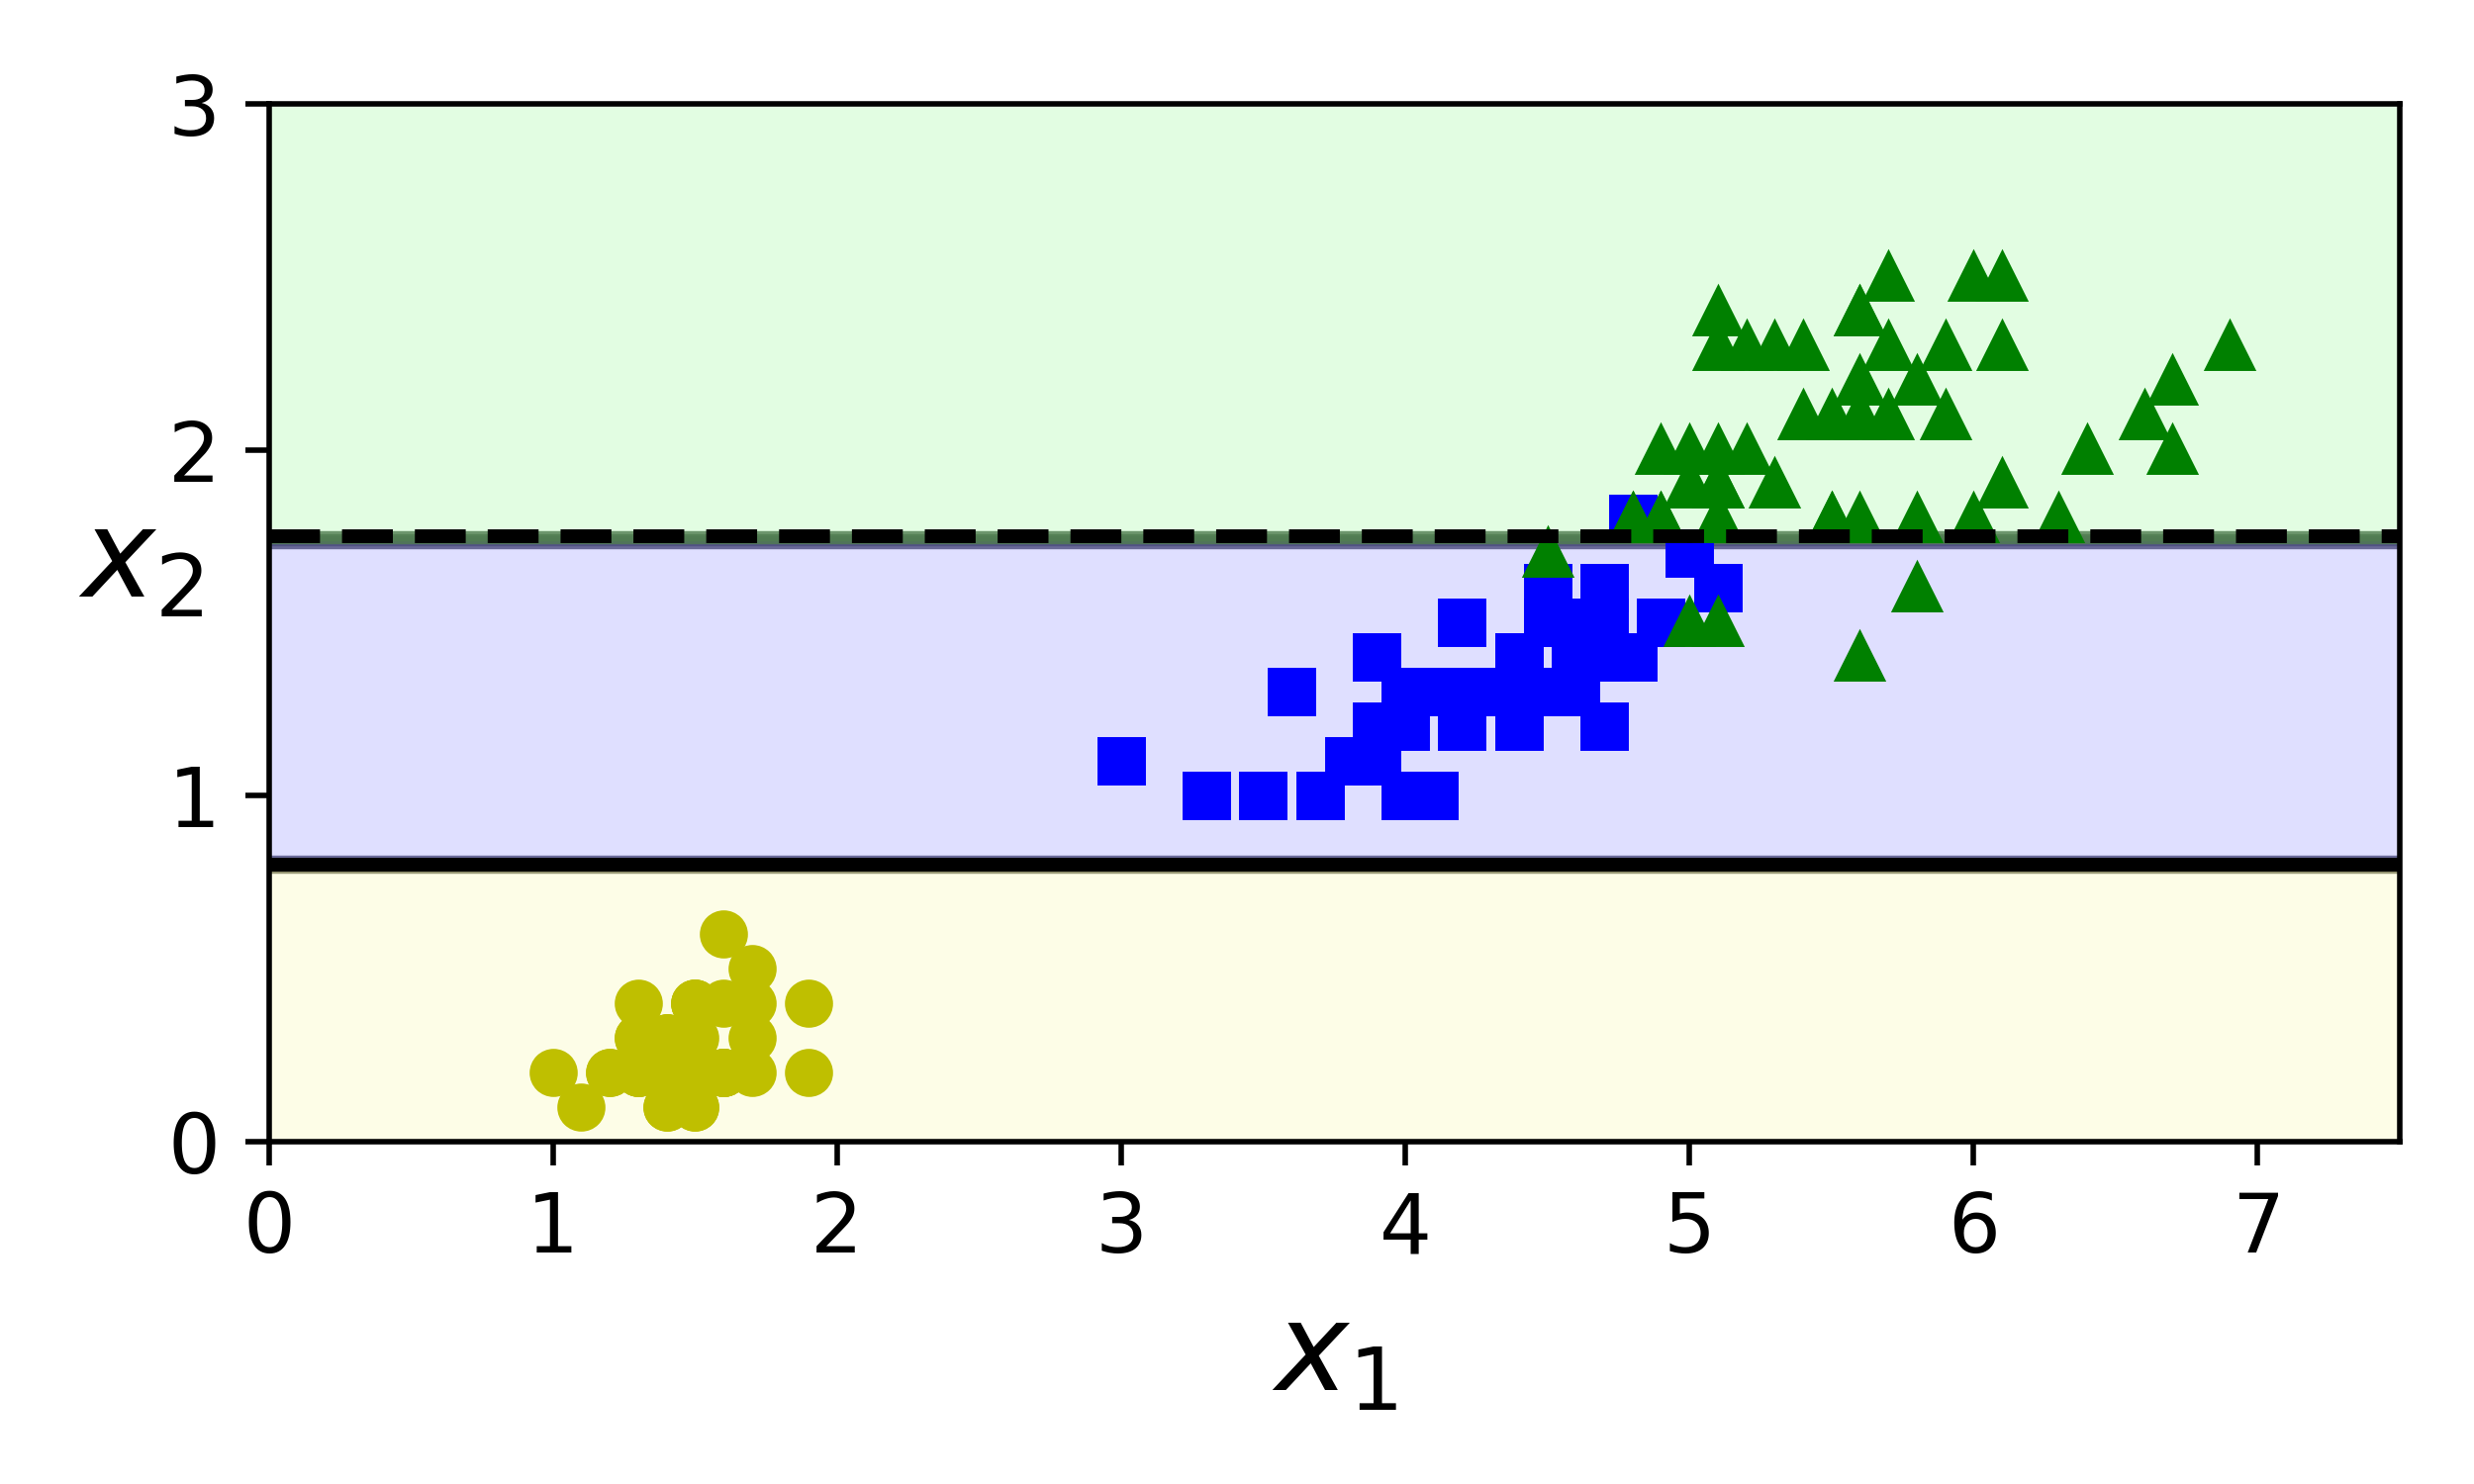
\includegraphics[width=7cm, height=7cm, keepaspectratio]{images/decision_trees_11.png}
\end{center}
\end{frame}

\end{document}















